% Section content template for individual Educative lessons
% This file contains the actual content for a specific section
% Generated from Educative API section content

% Section: Activity Diagram for LinkedIn
% Section ID: 5714015537070080
% Section Slug: activity-diagram-for-linkedin
% Generated: 2025-12-14T13:35:25.125235

Activity diagrams are an effective way to visualize the flow of messages between activities within a system. We can create various activity diagrams for LinkedIn. In this lesson, we'll create activity diagrams for the following two activities:

\begin{itemize}
\item
\protect\phantomsection\label{0OwK_s1h5tyxCfP5fzyRj}
Creating a new post.
\item
\protect\phantomsection\label{AI-Do5V4ViBcoNeVu9ilG}
\textbf{Activity challenge:} A user creates a page.
\end{itemize}

\subsection{Creating a new post}\label{02DW2fCHMhb0H4sI9iHN6}
\\
The states and actions involved in this activity diagram are provided below.

\subsubsection{States}\label{-M_Mez-ieFsKpylWJg_MF}
\\
\textbf{Initial state:} The user selects the new post option.
\\
\textbf{Final state:}~The post is published.

\subsubsection{Actions}\label{pzPQyoUugiMqKyHMzNV92}
\\
The user selects the ``New Post'' option, chooses the desired privacy setting, adds any necessary attachments, and then publishes the post.

\begin{figure}[htbp]
 \centering
 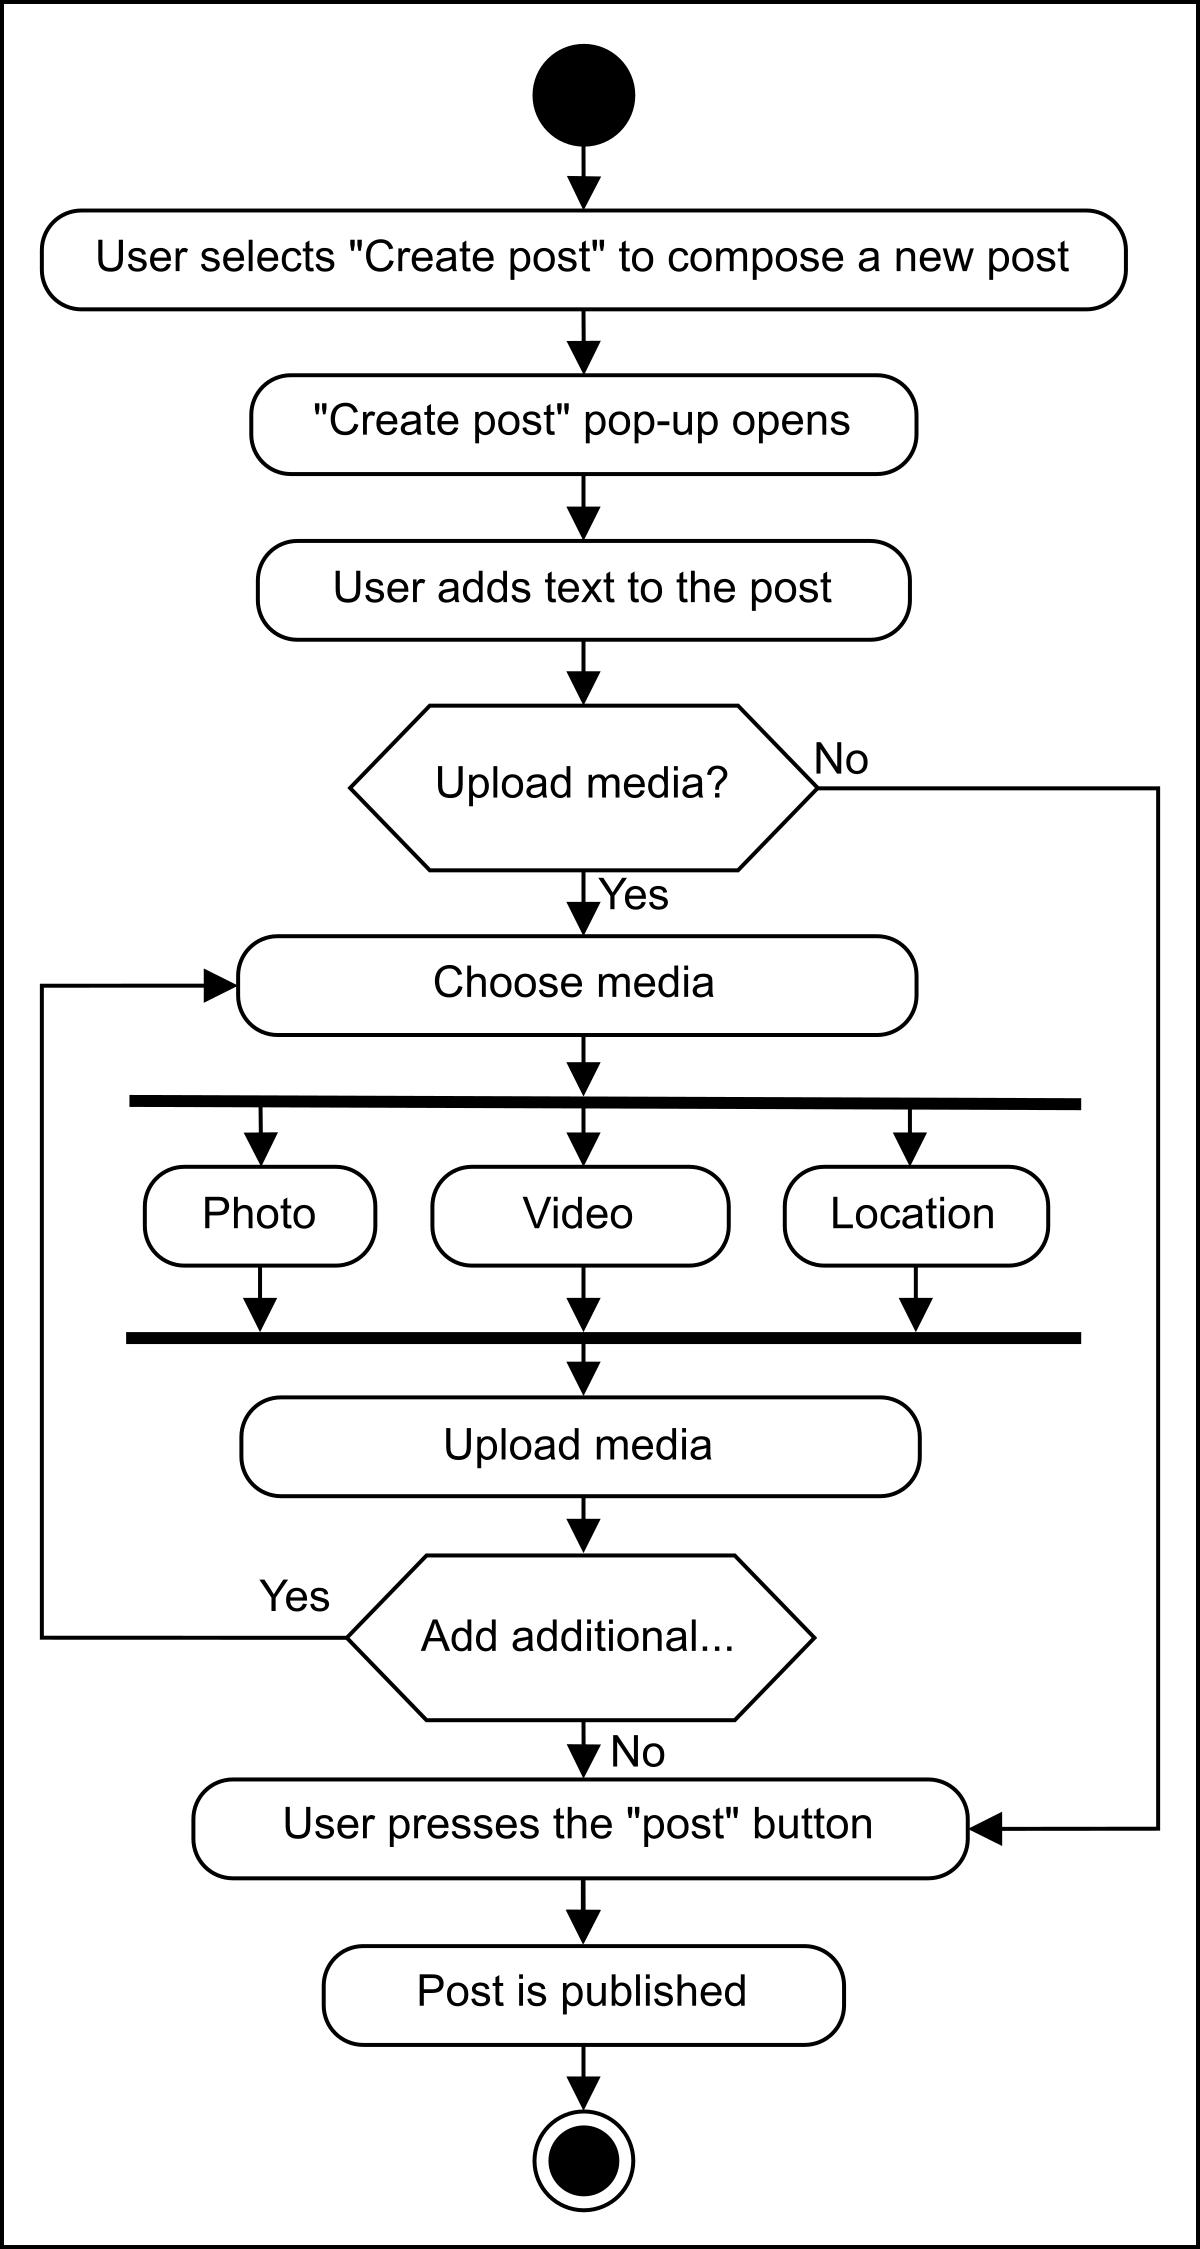
\includegraphics[width=0.5\textwidth]{Images/chapter_27/section_5714015537070080/5454920871575552.png}
 \caption{The activity diagram for a user creating a new post}
\end{figure}

\subsection{Activity challenge: A user creates a company page}\label{qeHLuVL5uq_Q40-lCVt8v}
\\
You'll help us create an activity diagram of a user creating a company page. A skeleton of the activity diagram is given below:

\begin{figure}[htbp]
 \centering
 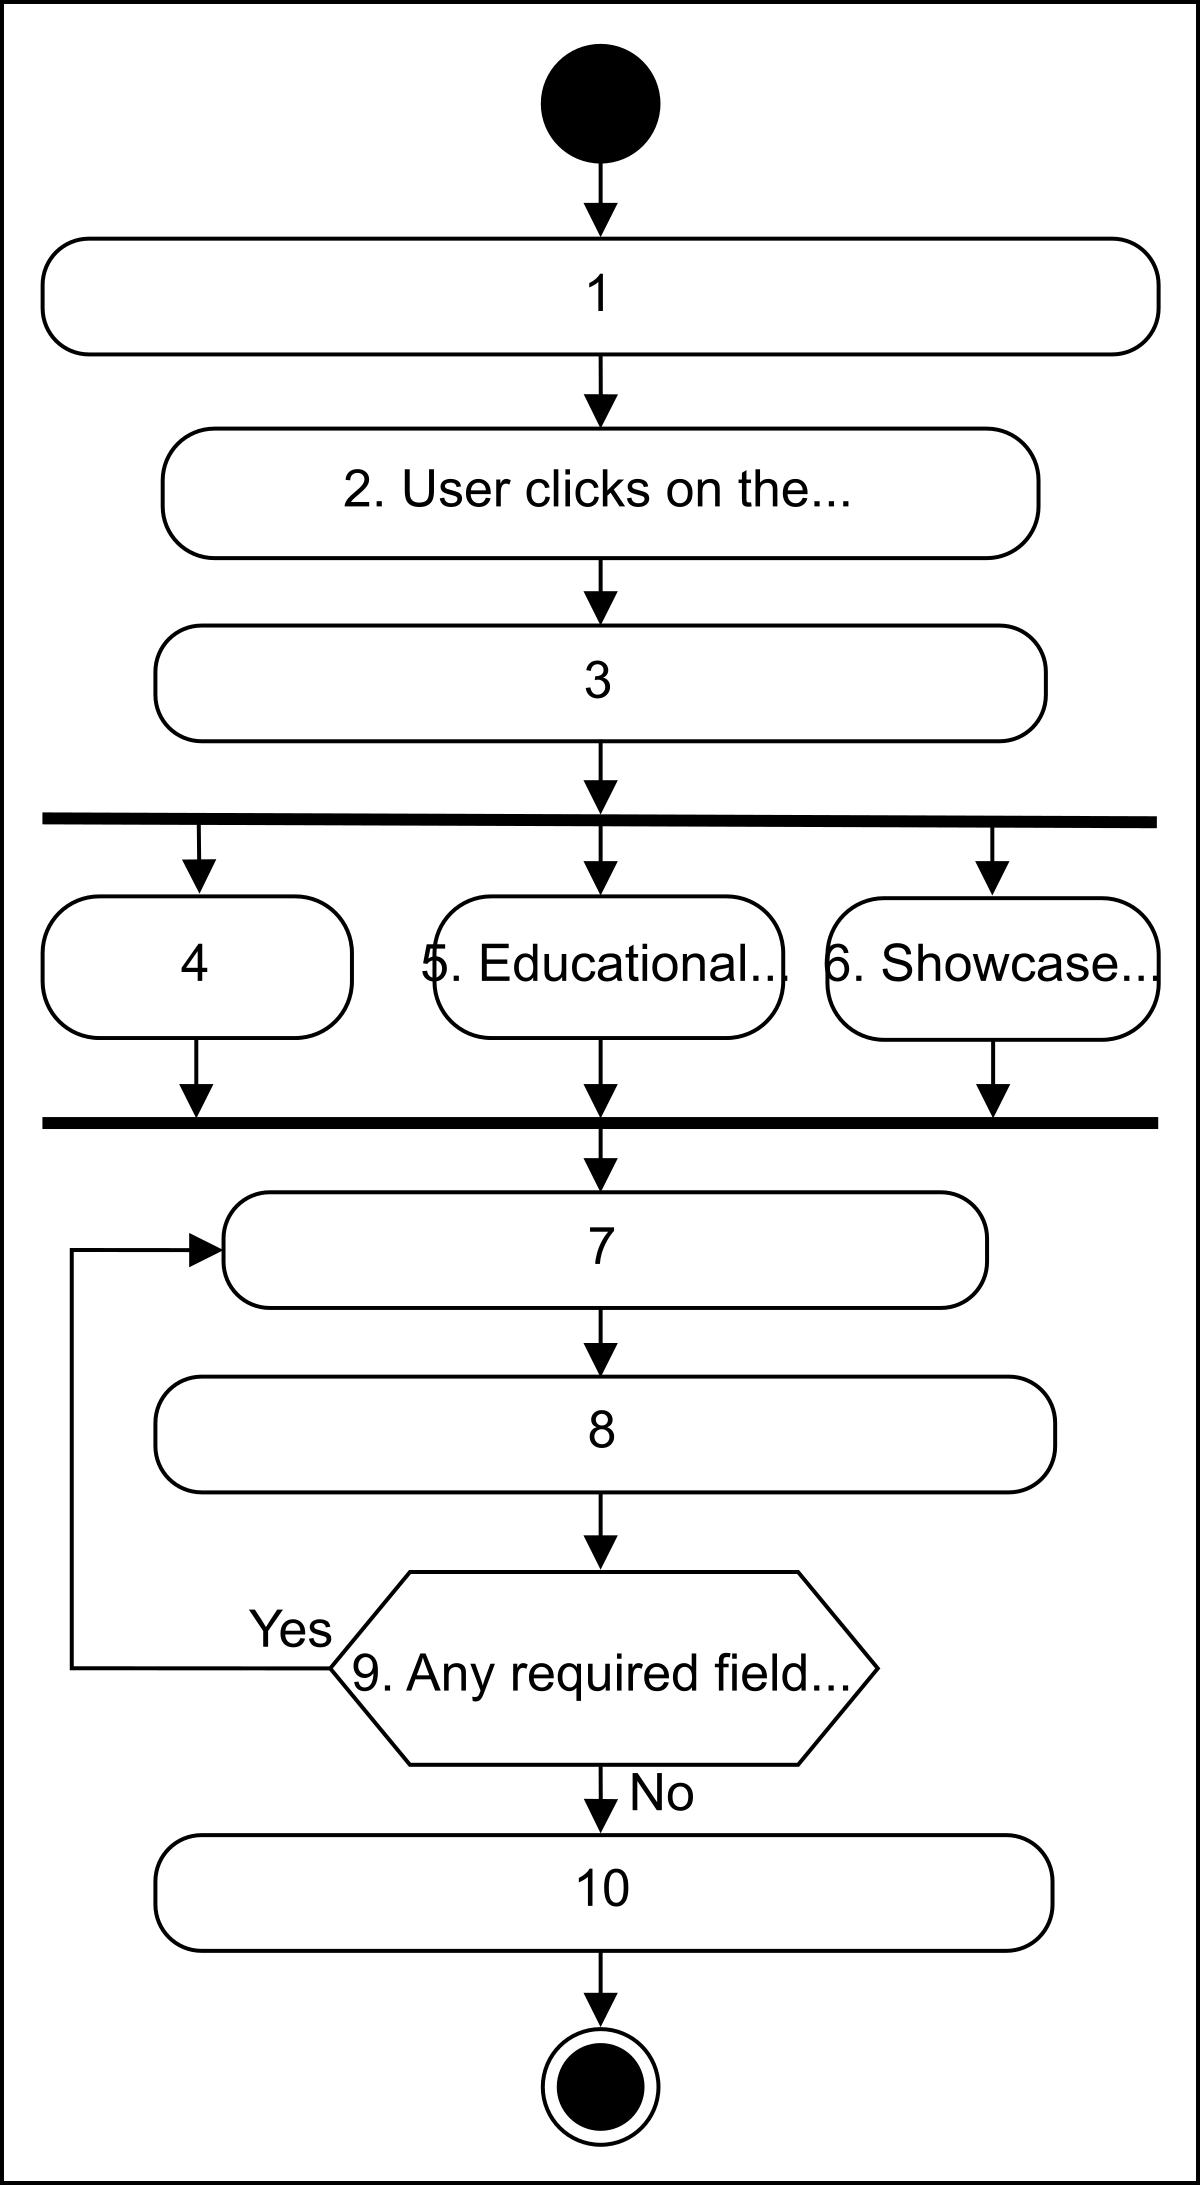
\includegraphics[width=0.5\textwidth]{Images/chapter_27/section_5714015537070080/6406542011400192.png}
 \caption{The activity diagram for a user creating a page}
\end{figure}

Notice that the actions in the diagram above are numbered from 1 to 10. The slots below represent the activities, and the arrows indicate the flow from one activity to another.
\\
Can you rearrange the slots below in the correct order they should appear in the activity diagram given above?
\begin{quote}
\textbf{Note:} If you're stuck, click the ``Show Solution'' button.
\end{quote}

Alternatively, you can click the ``Show complete diagram'' button below to see the complete activity diagram.

We've reviewed some of LinkedIn's activity diagrams. In the next lesson, we will present the code for our designed classes in some of the most popular languages.

% End of section content